\documentclass[preview,float]{standalone}
\usepackage{tikz}
\usetikzlibrary{hobby,decorations.markings}
\usepackage{graphicx}

\begin{document}
\begin{tikzpicture}
\coordinate (origo) at (0,0);

\draw [green,rotate around={50:(1.7,2.4)},->] (1.7,2.4) -- (3.3,2.4) node(mary)[above,right] {$V_x$};

\draw[green,
  postaction={
    decorate,
    decoration={
      markings,
      mark=between positions 0 and 1 step 0.33 with
      {
        \node[transform shape] {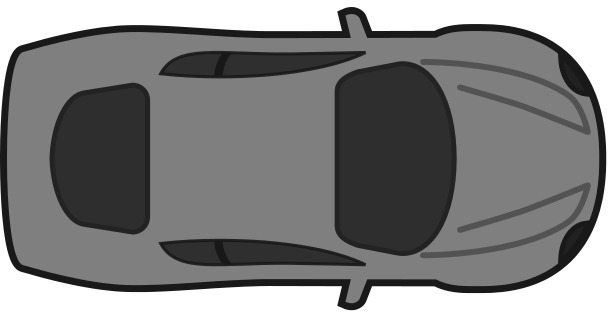
\includegraphics[width=1.5cm,angle=50]{car}};
      }
    }
  }
]
(1.7,2.4);

\draw[dashed]
(-1,0.7) parabola (5,5.0);
\draw
(-1,-0.7) parabola (5+1.4,5.0);
\draw
(-1,2.1) parabola (5-1.4,5.0);



\draw [red,rotate around={50+90:(1.7,2.4)},->] (2,2.4) -- (2.6,2.4) node[above] {$V_y$};

\draw [] (1.7,2.4) -- (2,1.8) node[below] {$e_1$};

\fill(2,1.8) circle (0.06);

\draw[dashed,thick,rotate around={30:(2,1.8)}] (2,1.8)--(4,1.6);

\draw[dashed,thick,rotate around={30:(1.7,2.4)}] (1.7,2.4)--(4-0.25,2.4) node(bob)[right]{};

\draw (2.63,2.93) arc (30:82-30:1) node[right]{$e_2$};

\draw[gray,->](2.2,1.5)--(4.5,0.4) node[below] {lateral deviation};
\draw[gray,->](2.4,3.3)--(1.1,4) node[above] {relative yaw angle};
\end{tikzpicture}
\end{document}